%!TEX root = ../main.tex
\section{Homework \thesection}

\subsection{Haar Wavelet Transform}
\begin{enumerate}
	\item Complete the Haar wavelet representation of following 1D image.
	Show the 8-element wavelet image.
	\begin{center}
	\begin{tabular}{|c|c|c|c|c|c|c|c|}
	\hline	2	&	4	&	2	&	0	&	6	&	2	&	1	&	7\\	\hline
	\end{tabular}
	\end{center}
	\item The wavelet basis provides a plausible means of compression by dropping certain coefficients.
	The most straightforward way of doing this is to cull the full set of coefficients of highest detail, \textit{i.e.}, set the coefficient layer immediately computed from 	the image to zero.
	For the 1D image above, compute the reconstructed image after compression.
	\item Consider a 1D image with \(2^n\) pixels.
	Assume that the bit-depth is \(b\) (grayscale image values with range 0 through \(2^b-1\)).
	Using the compression scheme above, derive an expression for the maximum error per pixel between the reconstructed image and original image.
	(The error here is computed by using \(\mathcal{L}^2\) norm).
\end{enumerate}
\subsubsection{Haar Wavelet Representation of 1D Image}
The only pixel with final coefficient layer is
\begin{center}
\begin{tabular}{|c|c|c|c|c|c|c|c|}
\hline	3	&	-1	&	1	&	0	&	-1	&	1	&	2	&	-3\\	\hline
\end{tabular}.
\end{center}

\subsubsection{Compression and Reconstruction}
By dropping the coefficients of highest detail
\begin{center}
\begin{tabular}{|c|c|c|c|}
\hline	-1	&	1	&	2	&	-3\\	\hline
\end{tabular},
\end{center}
the reconstructed image is
\begin{center}
\begin{tabular}{|c|c|c|c|c|c|c|c|}
\hline	3	&	3	&	1	&	1	&	4	&	4	&	4	&	4\\	\hline
\end{tabular}.
\end{center}
Note that it is the average of the adjacent pixels in the original image.

\subsubsection{Maximum Error of Reconstructed Image}
The maximum error occurs when the adjacent pixels are in pattern \(\left(0,2^{b}-1\right)\) or \(\left(2^{b}-1,0\right)\).
So the reconstructed image after compression is \(\frac{2^b-1}{2}\) in all \(2^n\) entries.
The \(\mathcal{L}^2\) norm is \(2^{\frac{n}{2}}\cdot\frac{2^b-1}{2}\).
For each pixel, the error is \[2^{-\frac{n}{2}-1}\cdot\left(2^b-1\right).\]


\subsection{House Number Classification}
Recall the eigenface example discussed in the class. Now apply the same technique to classify house numbers.\\
First of all, to get the basis of the digits, we use MNIST Dataset as training data.
MNIST is a large database of handwritten digits.
Download its training set images and labels from \href{http://yann.lecun.com/exdb/mnist/}{Yann LeCun's website}.
Every image contains a digit and has a size of \(28 \times 28\).
The original file is not in the standard image format (see how the pixels are arranged on the website).
You may search for helper functions to read the images and labels (one can be found on \href{http://ufldl.stanford.edu/wiki/index.php/Using_the_MNIST_Dataset}{this site}).\\
Then download the SVHN test images from \href{http://ufldl.stanford.edu/housenumbers/}{its official site}.
There are two formats of data, original images and cropped and centered images.
Format 1 (test.tar.gz) is what we are going to use for classification.
The annotation of images, including the labels and bounding boxes, are stored in digitStruct.mat, which can also be found in the downloaded folder.
See detailed description
about the format of the annotation on the \href{http://ufldl.stanford.edu/housenumbers/}{official site}.\\
You are required to implement a nearest neighbor classifier to recognize the house numbers for the first 300 images in the test dataset.
Make use of the bounding box information to crop the image to the region of a specific digit and resize it to \(28 \times 28\) (think about why).
Note that there may be multiple digits in the same image and they are classified one by one to form a house number.
Compare the house number generated by your program with the groundtruth and calculate the Number Error Rate and Digit Error Rate using the formula below.
\begin{align*}
	\text{Number Error Rate}
	&=\frac{\text{number of wrong house numbers}}{\text{total number of house numbers}}\\
	\text{Digit Error Rate}
	&=\frac{\text{number of wrong digits}}{\text{total number of digits in all images}}
\end{align*}
Visualize first 10 basis calculated from MNIST that are associated with 10 largest eigenvalues and attach the images to your pdf writeup.
Include one example of the house number that can be correctly classified and one example that fails.
Also, report the error rate as described above.
Submit the original program files to Canvas (do not include the dataset).
Add a readme file to clarify the usage of your code.

\subsubsection{Test on Training Dataset MNIST}
I use the 10-nearest-neighbor classifier and the error rate on MNIST is 4.8\%, \textit{i.e.}, 24 wrong classifications out of 500.
\subsubsection{Test on SVHN}
The digit error rate is 87.5\%, and the number error rate is 97\%.
Actually, only 9 housenumbers are correctly classified.
\begin{figure}[htbp]
	\centering
	\begin{subfigure}[t]{0.4\textwidth}
	    \centering
		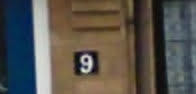
\includegraphics[width=0.8\textwidth]{hw4/problem2/23.png}
		\caption{Successful}\label{fig:16a}
	\end{subfigure}
	\qquad
	\begin{subfigure}[t]{0.4\textwidth}
	    \centering
		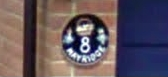
\includegraphics{hw4/problem2/53.png}
		\caption{Successful}\label{fig:16b}
	\end{subfigure}
	\qquad
	\begin{subfigure}[t]{0.4\textwidth}
	    \centering
		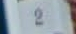
\includegraphics{hw4/problem2/66.png}
		\caption{Successful}\label{fig:16c}
	\end{subfigure}
	\qquad
	\begin{subfigure}[t]{0.4\textwidth}
	    \centering
		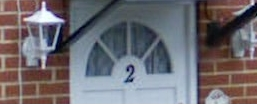
\includegraphics[width=0.6\textwidth]{hw4/problem2/97.png}
		\caption{Successful}\label{fig:16d}
	\end{subfigure}
	\qquad
	\begin{subfigure}[t]{0.4\textwidth}
	    \centering
		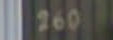
\includegraphics{hw4/problem2/24.png}
		\caption{Fail}\label{fig:16e}
	\end{subfigure}
	\caption{An example of successful classification}\label{fig:16}
\end{figure}
The successful classifications are all very clear, and most of them have only one digit, which makes it easier to classify.
The unsuccessful exmaples fail for multiple reasons: unclear boundary, noisy background, non-central alignment and non-upward orientation.
\lstinputlisting[style=Matlab-editor]{./hw4/problem2/knn.m}
\lstinputlisting[style=Matlab-editor]{./hw4/problem2/knn_test_mnist.m}
\lstinputlisting[style=Matlab-editor]{./hw4/problem2/knn_test_svhn.m}